\data{07/11/2019}
\chapter{Discriminative vs generative}
We talked a lot about generative model, that is assuming that there is a distribution governing the data. Moreover we doing generative model, we need to find all the possible weights, which can be pretty difficult, e.g., finding the argument of a website considering its links. In this case, instead of using a generative model, we could use a \textbf{discriminative model}, that is a model for which we care only about the boundaries. \newline
Discriminative learnings focuses on directly modeling the discriminant function. \newline
This approach is particularly used in classification since it allows to directly model the decision boundaries instead of inferring them from the modelled data distributions. \newline
\begin{center}
  \begin{tabular}{L{0.48\linewidth}|L{0.48\linewidth}}
    \multicolumn{1}{c|}{\textbf{PROS}}&\multicolumn{1}{c}{\textbf{CONS}}\\
    \hline
    When data are complex, modelling their distribution (generative learning) can be very difficult&The learned model is less flexible in its usage\\
    \hline
    If data discrimination is the goal, data distribution modeling is not needed&It does not allow to perform arbitrary inference tasks\\
    \hline
    Focuses parameters on the desired goal&It is not possible to efficiently generate new data from a certain class
  \end{tabular}
\end{center}
%
%
%
\section{Linear discriminative model}
The idea is to model a linear discriminative function by finding the right multiplicative factors, called \textbf{weights}, so that such function is a linear composition of the samples in the dataset:
\[f(\vect{x})=\vect{w}^T\vect{x}+w_0\]
$W_0$ is called the \textbf{bias} or \textbf{threshold}. \newline
This is the simplest function, which may mean that it is not always the best one, but in most cases is the best option available. \newline
%
%
\subsection{Linear Binary Classifier}
If we'd need to classify only over two possibility, then all we'd need is to have a binary classifier. The easiest thing to do is to consider the sign of the before formula:
\[f(\vect{x})=\sign(\vect{w}^T\vect{x}+w_0)\]
So if the result is less than 0, we have a class, if it's positive is the other class, while if is 0 that is the \textbf{decision boundary}. This is the set of points for which the discriminant function is 0 and is actually and \textit{hyperplane}. \newline
It follows that the weight vector $\vect{w}$ is orthogonal to the decision hyperplane:
\begin{proof}
\[\forall \vect{x},\vect{x}':f(\vect{x})=f(\vect{x}')=0\]
\[\vect{w}^T\vect{x}+w_0-\vect{w}^T\vect{x}'-w_0=0\]
\[\vect{w}^T(\vect{x}-\vect{x}')=0\]
\end{proof}
The value $f(\vect{x})$ of the function for a certain point $\vect{x}$ is called \textit{functional margin} and it can be seen as a confidence in the prediction: if the value is greatly bigger than the boundary, then we can be more confident regarding the decision. \newline
The distance from $\vect{x}$ to the hyperplane is called \textit{geometric margin}
\[r^x=\frac{f(\vect{x})}{\vert\vert\vect{w}\vert\vert}\]
It is a normalize version of the functional margin w.r.t. the weights. \newline
The distance from the origin to the hyperplane is:
\[r^0=\frac{f(\vect{0})}{\vert\vert\vect{w}\vert\vert}=\frac{w_0}{\vert\vert\vect{w}\vert\vert}\]
\begin{center}
  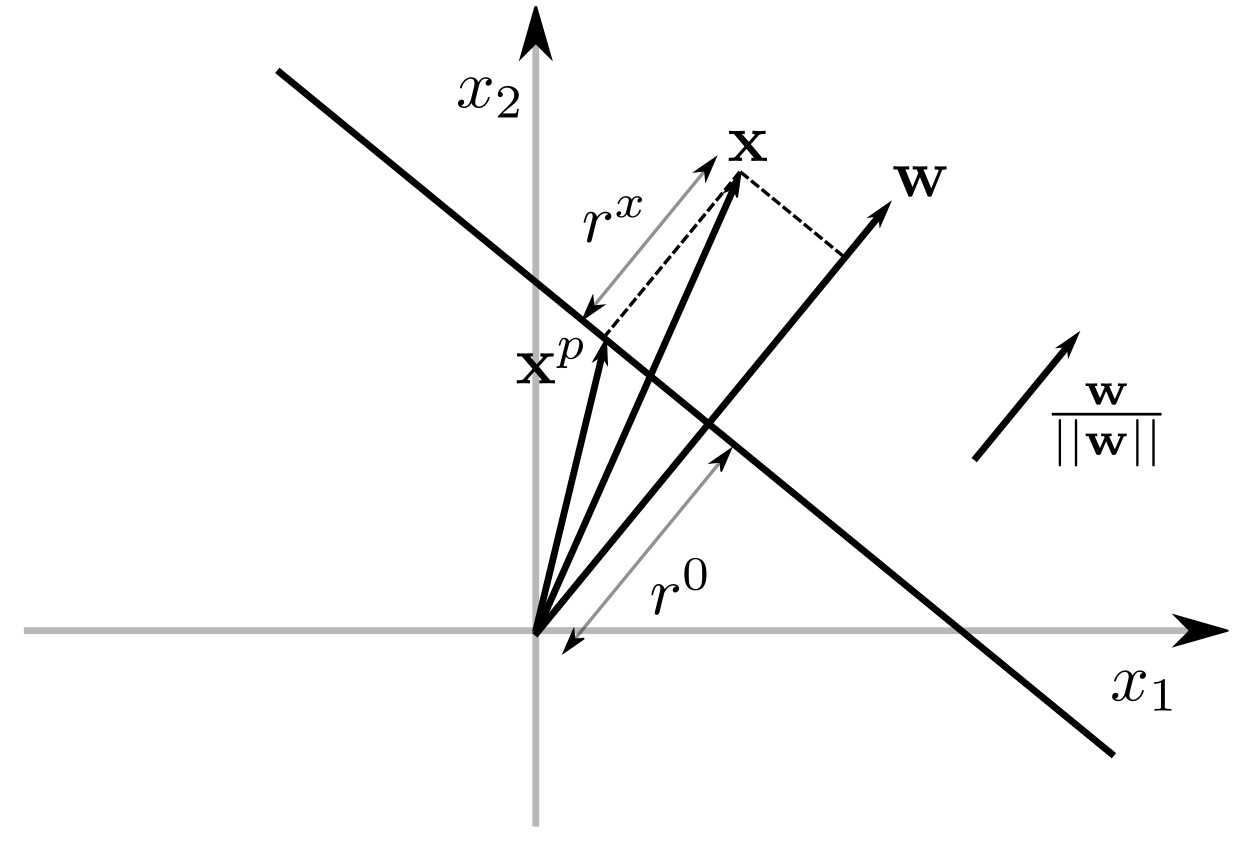
\includegraphics[width=0.6\linewidth]{LinBinClas}
\end{center}
\begin{proof}
A point $\vect{x}$ can be expressed by its projection $\vect{x}^p$ on the hyperplane $H$ plus its distance to the hyperplane times the unit vector $\myfrac{\vect{w}}{\vert\vert\vect{w}\vert\vert}$ in that direction:
\[\vect{x}=\vect{x}^p+r^x\frac{\vect{w}}{\vert\vert\vect{w}\vert\vert}\]
Since the point is on the hyperplane, then we have:
\[f(\vect{x}^p)=0\]
Now we know that:
\[f(\vect{x})=\vect{w}^T\vect{x}+w_0\]
By writing $vect{x}$ as the projection we have:
\[
  \begin{array}{ll}
    f(\vect{x}&=\vect{w}^T\left(\vect{x}^p+r^x\frac{\vect{w}}{\vert\vert\vect{w}\vert\vert}\right)+w_0\\
              &=\vect{w}^T\vect{x}^p+w_0+r^x\vect{w}^T\frac{\vect{w}}{\vert\vert{\vect{w}\vert\vert}}
  \end{array}
\]
But $\vect{w}^T\vect{x}^p+w_0=f(\vect{x}^p)$ which is 0:
\[f(\vect{x})=r^x\vect{w}^T\frac{\vect{w}}{\vert\vert\vect{w}\vert\vert}=r^x\vect{w}^T\frac{\vect{w}}{\vert\vert\vect{w}\vert\vert}\]
The product of the transpose for the vector is the square of the norm, hence:
\[f(\vect{x})=r^x\vert\vert\vect{w}\vert\vert\]
By inverting we have:
\[r^x=\frac{f(\vect{x})}{\vert\vert\vect{w}\vert\vert}\]
\end{proof}



\section{Perceptron -- A Biological Approach}
The linear classifier, called \textbf{perceptron}, takes inspiration from the brain which is composed of densely interconnected networks of neurons. \newline
Each neuron is made out of:
\begin{itemize}
  \item \textit{Soma}: a central body containing the nucleus;
  \item \textit{Dendrites}: they surround the soma and are a set of filaments departing from the body;
  \item \textit{Axon}: the longest dendrite;
  \item \textit{Synapses}: connections between dendrites and axons from other neurons. 
\end{itemize}
\begin{center}
  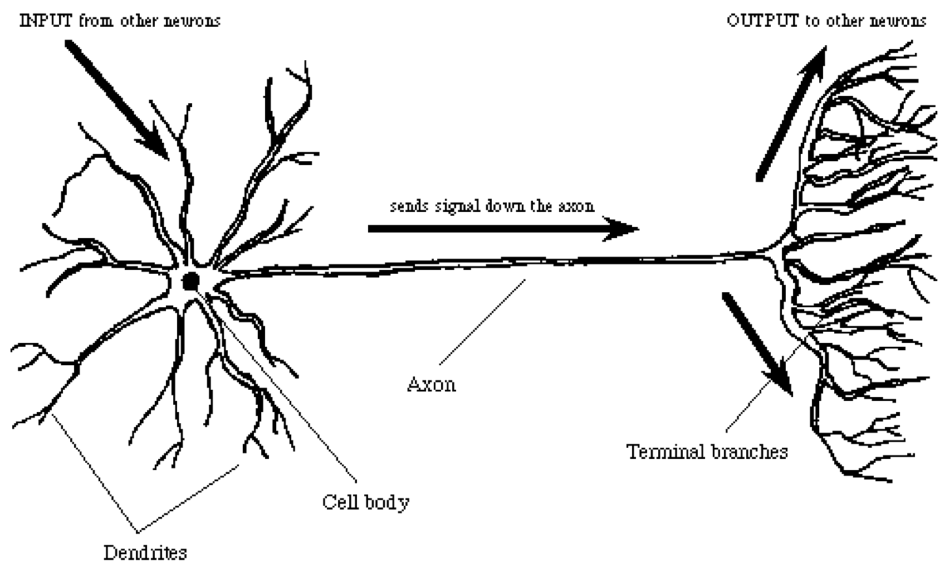
\includegraphics[width=0.7\linewidth]{Neuron}
\end{center}
Electrochemical reactions allows the signals to propagate in the brain via axons, synapses and dendrites. \newline
Each synapse can either \textit{excite} or \textit{inhibit} a neuron potential: once a neuron potential exceeds a certain threshold, a signal is generated and transmitted along the axon. \newline
What it's possible to do is to create a classifier that behaves similarly to how neurons do. This classifier is called \textbf{perceptron}. \newline
To compare a perceptron with a neuron we can say that the dendrites are actually the classes present in the inputs, while the synapses are the functions, called \textbf{activation functions}, that discriminate between the classes based on a certain threshold. \newline
Note that a weight is associated to each feature and the results are summed before being sent to the activation function.  
\begin{figure}
  \centering
  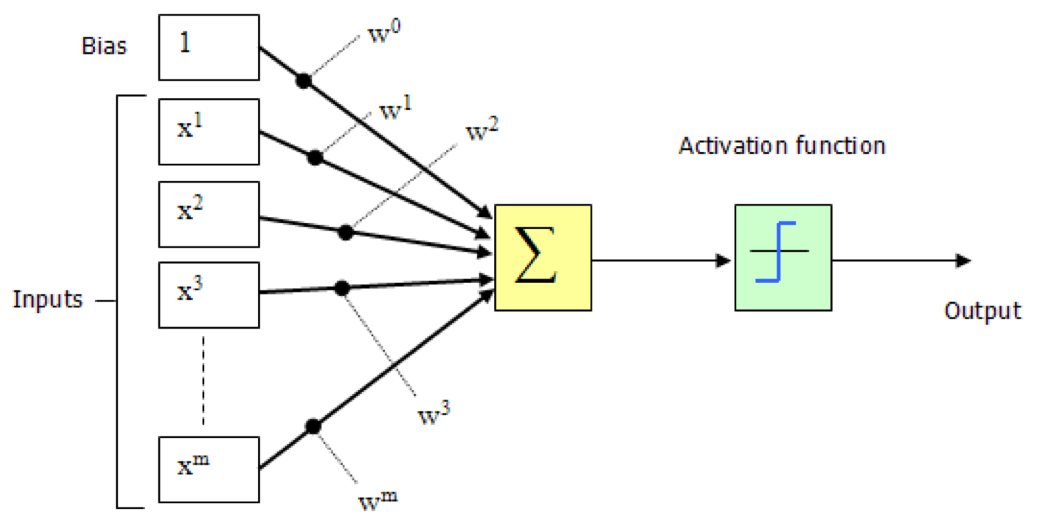
\includegraphics[width=0.7\linewidth]{Perceptron}
  \caption{The scheme of a perceptron.}
  \label{fig:Perceptron}
\end{figure}
The simplest formulation for a perceptron is a binary classifier for which the activation function is a sign function:
\begin{equation}
  f(\vect{x})=\sign{\vect{w}^T\vect{x}+w_0}
  \label{eq:BinaryPerceptron}
\end{equation}
In this case the threshold would be 0: if the value is bigger, then we can classify the sample with a class, if the value is smaller, then we can classify the sample with the other class. \newline
A \textit{linear classifier} (perceptron) can \textit{linearly} separate classes that are \textit{linearly separable}, for example boolean functions such as AND, OR, NOT, NAND since in this case two features can be either 1 or 0. For instance, if we consider the OR the result can be either positive or negative and hence easily separable by a line. The same can be said for the AND and the NOT. But if we were to consider the XOR, then dividing by an hyperplane is not possible, hence the XOR is not linear separable function.
\begin{center}
\begin{figure}[htp]
  \begin{subfigure}{0.31\linewidth}%OR
      \centering
      \includegraphics[width=\linewidth]{OR.tikz}  
      \caption*{OR}
  \end{subfigure}
  \hspace{0.01\linewidth}
  \begin{subfigure}{0.31\linewidth}%OR
      \centering
      \includegraphics[width=\linewidth]{AND.tikz}  
      \caption*{AND}
  \end{subfigure}
  \hspace{0.01\linewidth}
  \begin{subfigure}{0.31\linewidth}%OR
      \centering
      \includegraphics[width=\linewidth]{XOR.tikz}  
      \caption*{XOR}
  \end{subfigure}
  \caption{It's possible to notice that while both AND and OR are easily linearly separable, the same cannot be said for the XOR since it's not possible to find a line that separate correctly the positives from the negatives.}
  \label{fig:BooleanPerceptron}
\end{figure}
\end{center}
To solve the XOR we can use a multilevel perceptron. Indeed, we know that 
\[A\oplus B=(A\wedge not B)\vee (not A\wedge B)\]
So we could compute the parenthesis separately first and the unite them via an OR. 
\begin{center}
  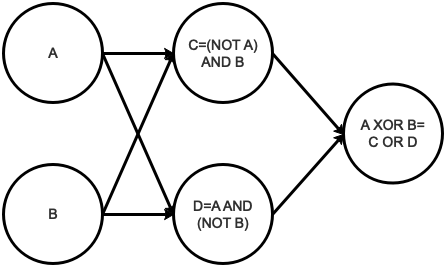
\includegraphics[width=0.5\linewidth]{XORPerceptron}
\end{center}
This could be true for every boolean formula: all of them could be learned by a two layer perceptron since all boolean formulas can be expressed in conjunctive or disjunctive normal formulas. Why then do we need multi strata deep networks instead of using only two? Because the conjunctive, disjunctive, normal formulas are exponentially in term of number of neurones. \newline
In the Figure~\ref{fig:Perceptron}, it's possible to notice that also a bias is present. Such bias is set to 1 by default and its weight will let it be useful by learning the actual value. Moreover, this value allows us to rewrite Equation~\ref{eq:BinaryPerceptron} as augmented vectors:
\begin{equation*}
  f(\vect{x})=\sign{\vect{\widehat{\vect{w}}}^T\widehat{\vect{x}}}
\end{equation*}
where:
\[
  \widehat{\vect{w}}=\begin{pmatrix}w_0\\\vect{w}\end{pmatrix}\qquad
  \widehat{\vect{x}}=\begin{pmatrix}1\\\vect{x}\end{pmatrix}\qquad
\]
From now one all the formula will include bias and weight without specifying.\newline
%
%
%
\section{Parameter Learning}
Our goal now is to optimize a function of the parameters in the same way we did for maximum likelihood for probability distributions. \newline
Since the weights are learned from the data $\mathcal{D}$, then an error function, e.g., the loss function $l$, will do the deed:
\[E(\vect{w};\mathcal{D})=\Sum_{(\vect{x},y)\in\mathcal{D}}l(\vect{y},f(\vect{x}))\]
This though can lead to overfitting since the algorithm could simply memorize all the training examples. This actually is not a problem with linear classifiers, but with more difficult systems, this solution is not sufficient. 
%
%
\subsection{Gradient Descent -- Batch Training} %TODO listen this lesson back
Now let's suppose we know the loss function we want to use, we can try to do error minimization by changing the weighs. One way to approach this problem is gradient descend. Let's suppose we have just one parameter and the error function over the parameter is the following:
\begin{center}
  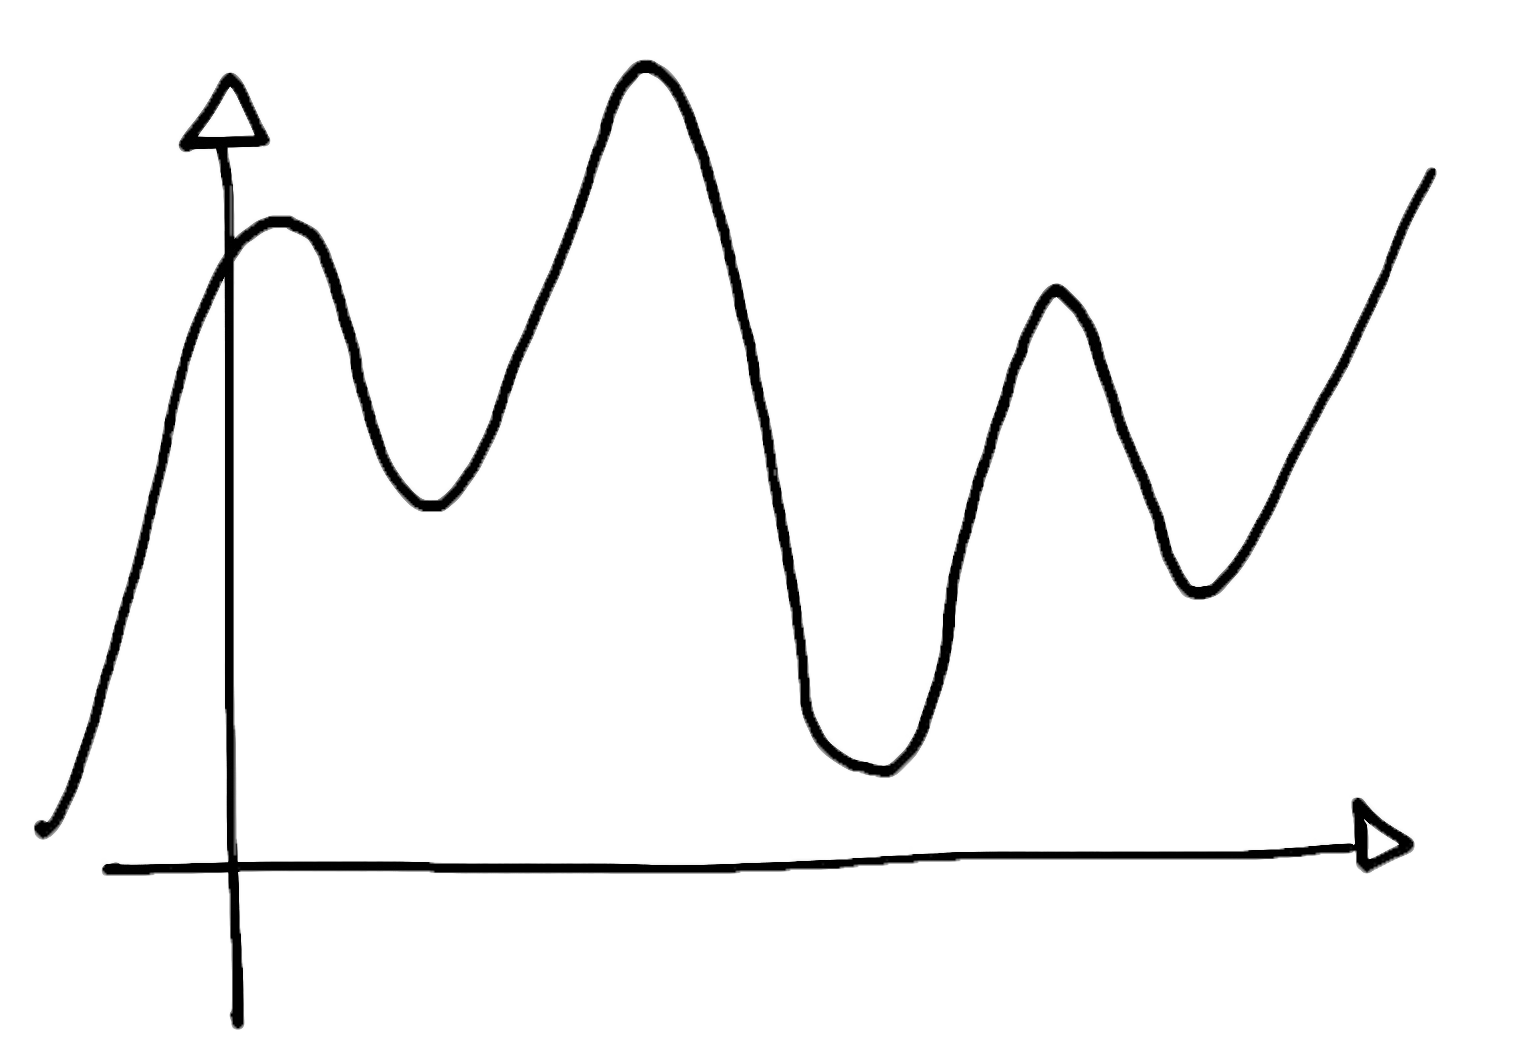
\includegraphics[width=0.6\linewidth]{GradientDescentExample1}
\end{center}
To minimise it, we start from $\vect{w}=0$, then we compute the gradient and move opposite of the gradient (otherwise we'd maximise). Then we compute the new weights as:
\[\vect{w}=\vect{w}-\eta\nabla E(\vect{w};\mathcal{D})\]
where $\eta$ is the learning rate and tells the algorithm how much it needs to move on the graph each time. \newline
After recomputing the weights, we repeat the procedure until the gradient is approximately zero. Mind that with this approach we reach just a local minimum. The learning rate $\eta$ plays an important role in finding the local minimum: 
\begin{itemize}
  \item Too low: means a slow convergence;
  \item Too high: means jumping around the curve.
\end{itemize}
There exist also techniques to adaptively modify $\eta$.
Let:
\[E(\vect{w};\mathcal{D})=\Sum_{(\vect{x},y)\in\mathcal{D}_E}-yf(\vect{x})\]
Where $\mathcal{D}_E$ is the set of current training errors for which:
\[yf(\vect{x})\leq 0\]
The error is the sum of the functional margins of incorrectly classified examples. \newline
The error gradient is:
\begin{equation*}
  \begin{array}{ll}
    \nabla E(\vect{w};\mathcal{D})&=\nabla\Sum_{(\vect{x},y)\in\mathcal{D}_E}-yf(\vect{x})\\
                                  &=\nabla\Sum_{(\vect{x},y)\in\mathcal{D}_E}-y(\vect{w}^T\vect{x})\\
                                  &=\Sum_{(\vect{x},y)\in\mathcal{D}_E}-y\vect{x}
  \end{array}
\end{equation*}
The amount of update is:
\[-\eta\nabla E(\vect{w};\mathcal{D})=\eta\Sum_{(\vect{x},y)\in\mathcal{D}_E}-y\vect{x}\]
Hence the update of the weights will be:
\[\vect{w}=\vect{w}+\eta \Sum_{(\vect{x},y)\in\mathcal{D}_E}-y\vect{x}\]
%In perceptron we use a confident margin: we do not take the sign of $f(x)$ but we multiply $f(x)$ with y, so the bigger the result the bigger the error.\newline 
This is called batch training because every step we compute the error on the entire training set.
%
%
\subsection{Stochastic Perceptron Training Rule}
In this version, each time we have a training error we make a gradient step: if the sample was correctly classified then ok, otherwise we move with the gradient and recompute the weights. The algorithm works as follows:
\begin{itemize}
  \item Initialize the weights randomly;
  \item Iterate until all examples are correctly classified:
    \begin{itemize}
      \item For each incorrectly classified training example $(\vect{x},y)$ update the weight vector:
        \[\vect{w}=\vect{w}+\eta y\vect{x}\]
    \end{itemize}
\end{itemize}
This is called stochastic perceptron and is usually pretty fast. In some cases it allows to avoid local minima since each time the gradient function is a little different, hence the algorithm is guided by various gradients for each training examples.\newline
What it basically does is to rotate the separating hyperplane until all the errors disappear.
\begin{center}
  \begin{minipage}{\linewidth}
    \begin{minipage}{0.48\linewidth}
      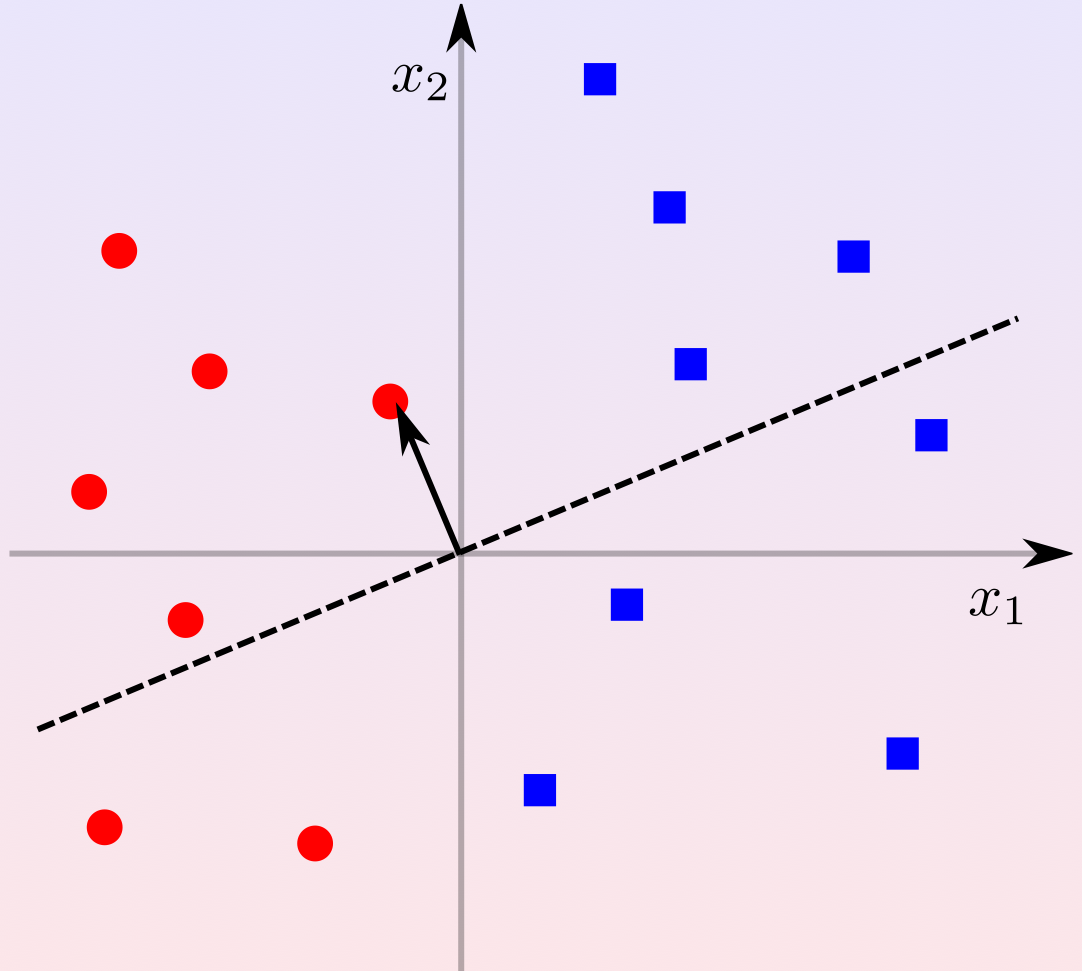
\includegraphics[width=\linewidth]{StochasticGradientDescent1}
    \end{minipage}
    \hspace{0.02\linewidth}
    \begin{minipage}{0.48\linewidth}
      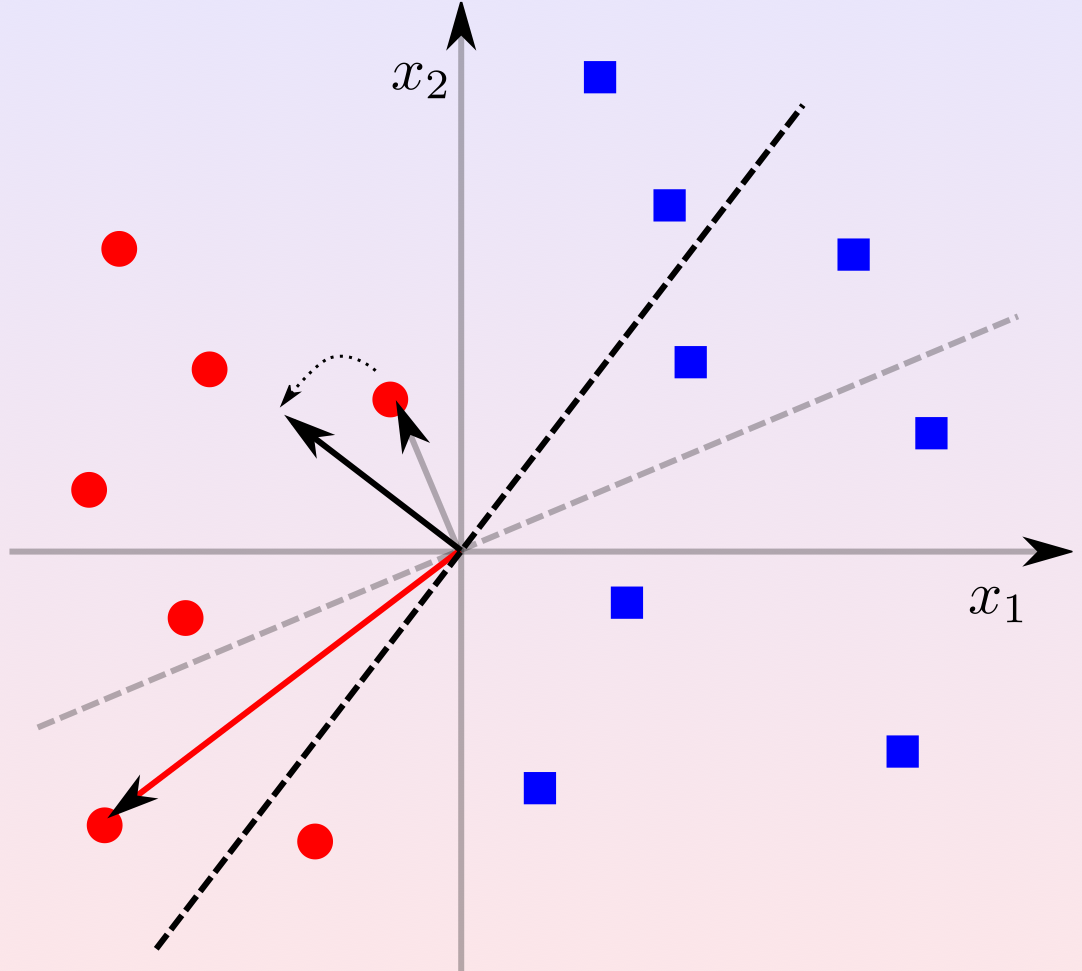
\includegraphics[width=\linewidth]{StochasticGradientDescent2}
    \end{minipage}\\
    \vspace{0.1cm}\\
    \begin{minipage}{0.48\linewidth}
      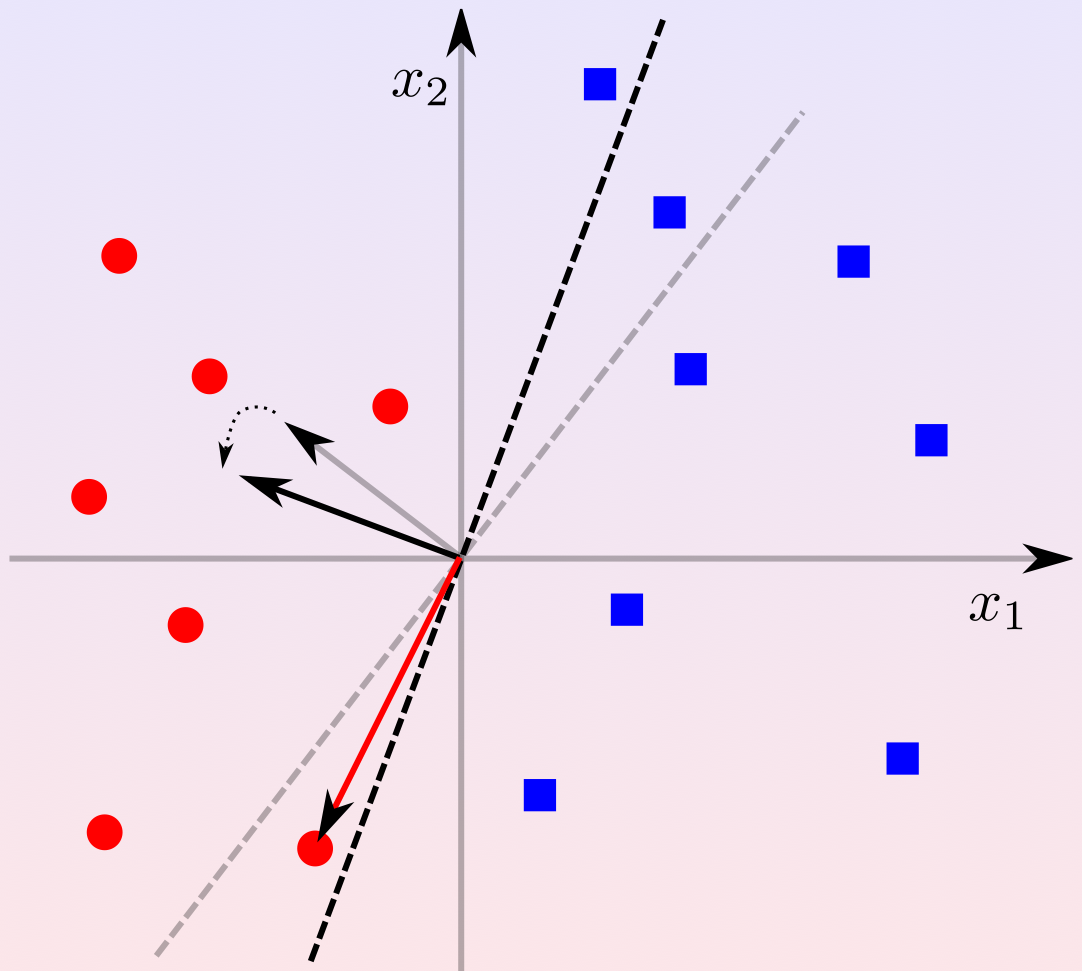
\includegraphics[width=\linewidth]{StochasticGradientDescent3}
    \end{minipage}
    \hspace{0.02\linewidth}
    \begin{minipage}{0.48\linewidth}
      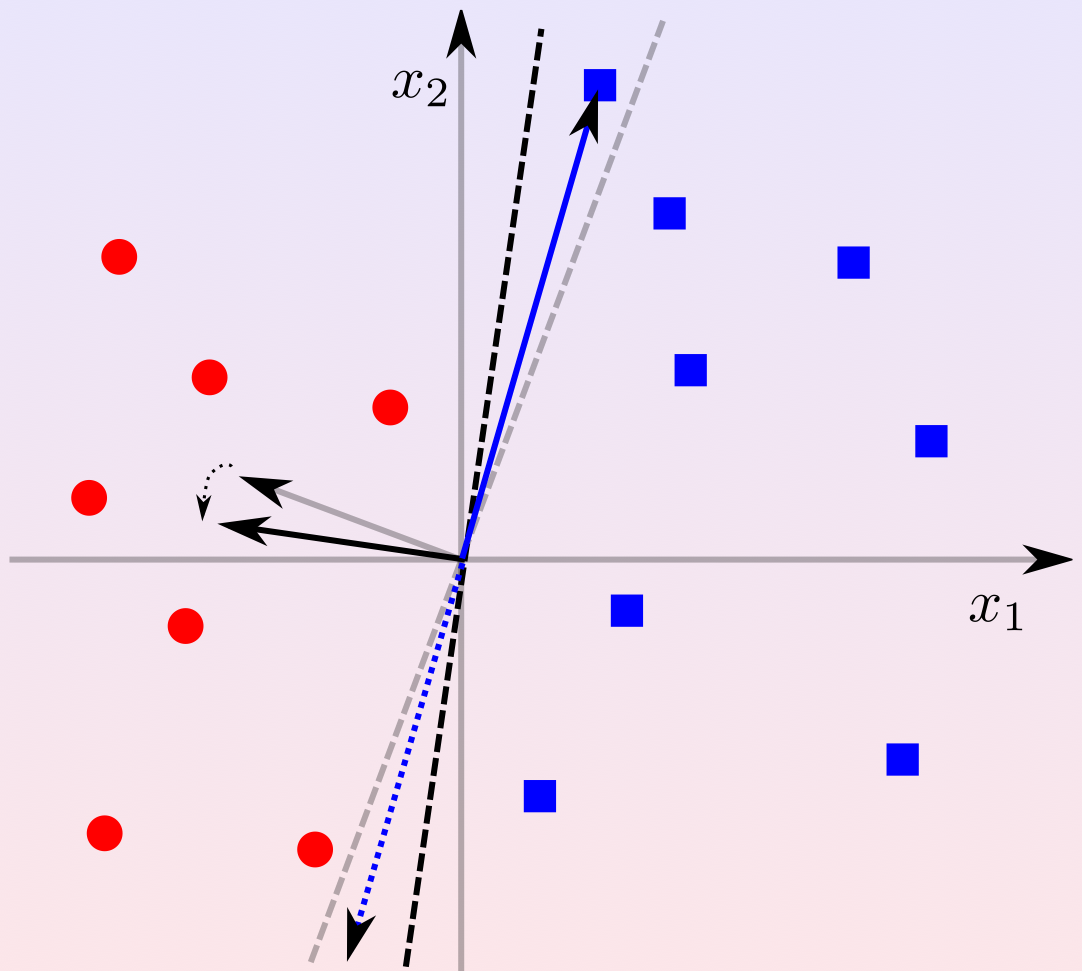
\includegraphics[width=\linewidth]{StochasticGradientDescent4}
    \end{minipage}
  \end{minipage}
\end{center}
%
%
%
\section{Regression with Perceptrons -- Exact Solution}
With linear predictors we can also do regression other the classification. \newline
Let's say we have $n$ examples $\vect{x}_i$ and that each example has $\vert \vect{x}_i\vert$ features, formally let $X\in\mathbb{R}^n\times\mathbb{R}^d$ be the input matrix, $X=[\vect{x}^1,\hdots,\vect{x}^n]^T$ for $n=\vert\mathcal{D}\vert$ and $d=\vert\vect{x}\vert$. \newline
Let $\vect{y}\in\mathbb{R}^n$ be the output training matrix (i.e., $y_i$ is output for example $\vect{x}_i$. The desired output is an $n$-dimensional vector of real values. \newline
Given that the regression learning function could be state as a set of linear equations:
\[X\vect{w}=\vect{y}\]
The perfect regression would be:
\[\forall i, y_i=\vect{w}^T\vect{x}_i\]
\[\vect{w}=X^{-1}\vect{y}\]
But this doesn't work since $X$ is not revertible in many cases. Moreover, the system of equations is usually overdetermined, that is there are more equations than unknowns. This means that usually there is no exact solution: we should forget about having an exact solution, but rather trying to minimize the error.
%
%
\subsection{Mean Squares Error}
We shall resort to loss minimization. The standard loss for regression is the mean squared error:
\[E(\vect{w};\mathcal{D})=\Sum_{(\vect{x},y)\in\mathcal{D}}(y-f(\vect{x}))^2=(\vect{y}-X\vect{w})^T(\vect{y}-X\vect{w})\]
For this we also have a closed form and it can be solved by gradient descent, which make it usable also for classification loss. \newline
The closed form can be computed by setting the gradient descent to 0:
\begin{equation*}
  \begin{array}{ll}
    \nabla E(\vect{w};\mathcal{D})&=\nabla (\vect{y}-X\vect{w})^T(\vect{y}-X\vect{w})\\
                                  &=2(\vect{y}-X\vect{w})^T(-X)=0\\
                                  &=-2\vect{y}^TX+2\vect{w}^Tx^TX=0\\
    \vect{w}^TX^TX                &=\vect{y}^TX\\
    X^TX\vect{w}                  &=X^T\vect{y}\\
    \vect{w}                      &=(X^TX)^{-1}X^T\vect{y}
  \end{array}
\end{equation*}
The part $(X^TX)^{-1}X^T$ is called \textit{left-inverse}: if $X$ is square and nonsingular, inverse and left-inverse coincide and the MSE solution corresponds to the exact one. \newline
The left-inverse exists provided $(X^TX)\in\mathbb{R}^{d\times d}$ is full rank, that is the features are linearly independent. If not we could simply remove the redundant ones and have a left-inverse. \newline
This said, the solution via gradient descent is usually the most efficient. We descend for each weight $w_i$ so that we can quantify the next weight variation. The following operations are meant to be executed on the full vector of the weights. 
\[
  \begin{array}{ll}
    \frac{\delta E}{\delta\vect{w}_i}&=\frac{\delta}{\delta\vect{w}_i}\frac{1}{2}\Sum_{(\vect{x},y)\in\mathcal{D}}(y-f(\vect{x}))^2\\
                                     &=\frac{1}{2}\Sum_{(\vect{x},y)\in\mathcal{D}}\frac{\delta}{\delta\vect{w}_i}(y-f(\vect{x}))^2\\
                                     &=\frac{1}{2}\Sum_{(\vect{x},y)\in\mathcal{D}}2(y-f(\vect{x}))\frac{\delta}{\delta\vect{w}_i}(y-\vect{w}^T\vect{x})\\
                                     &=\Sum_{(\vect{x},y)\in\mathcal{D}}(y-f(\vect{x}))(x_i)\\
  \end{array}
\]
%
%
%
\section{Multiclass Classification}
We'll briefly see two possible approaches.
%
%
\subsection{Multiclass Classification -- One-VS-All}
In this case the idea is to learn a binary classifier for each class: or the example belongs to said class, or it does not an belongs to another class. \newline
The idea is to predict a new example in the class with maximum functional margin. \newline
The decision boundaries for which $f_i(\vect{x})=f_j(\vect{x})$ are pieces of hyperplanes:
\[\vect{w}_i^T\vect{x}=\vect{w}_j^T\vect{x}\]
\[(\vect{w}_i-\vect{w}_j)^T\vect{x}=0\]
\begin{center}
  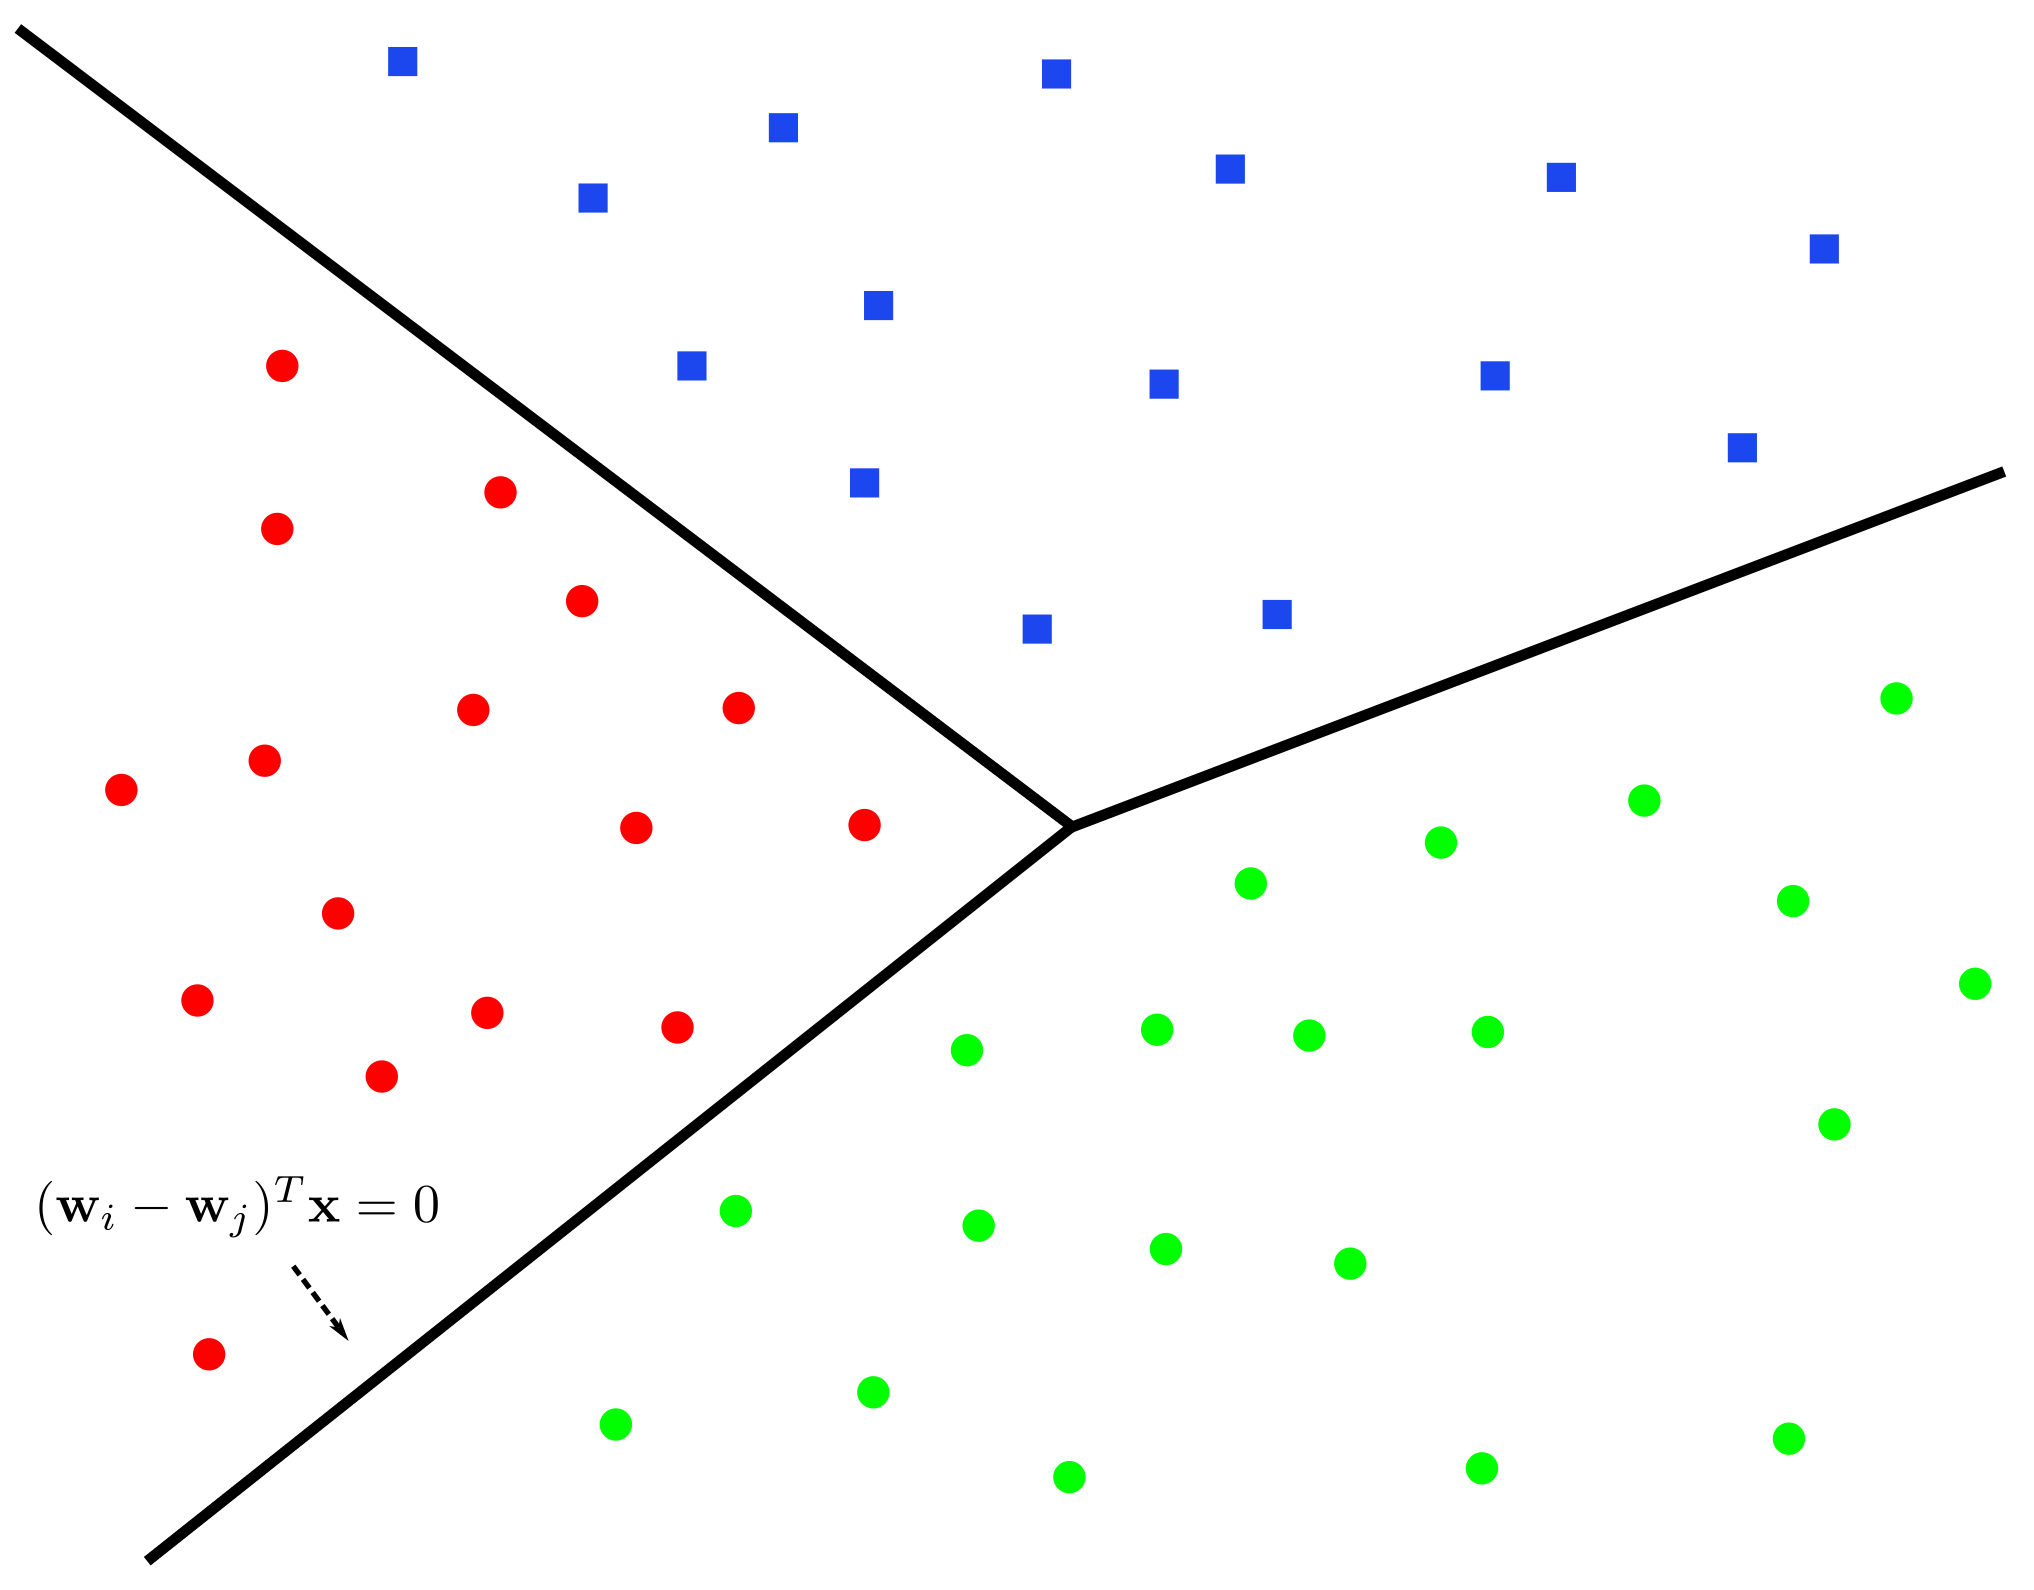
\includegraphics[width=0.7\linewidth]{MulticlassClassifcationOneVSAll}
\end{center}
%
%
\subsection{Multiclass Classification -- All-Pairs}
In this case the classes are paired and one binary classifier is associated to each pair:
\begin{itemize}
  \item Positive examples are from class A;
  \item Negative examples are from class B.
\end{itemize}
The new example is predicted as belonging to a class when it wins the largest number of pairwise classifications. 
%
%
%
\section{Generative Linear Classifiers}
In Gaussian distributions, the boundaries are obtained when the covariance is shared among classes: $\sigma_i=\sigma$. 
We could use Naive Bayes as a classifier:
\[f_i(\vect{x})=P(\vect{x}\vert y_i)P(y_i)=\Prod_{j=1}^{\vert\vect{x}\vert}\Prod_{k=1}^K\theta_{ky_i}^{z_k(x[j])}\frac{\vert\mathcal{D}_i\vert}{\vert\mathcal{D}\vert}\]
\[f_i(\vect{x})=\Prod_{k=1}^K\theta_{ky_i}^{N_{k\vect{x}}}\frac{\vert\mathcal{D}_i\vert}{\vert\mathcal{D}\vert}\]
Where $N_{k\vect{x}}$ is the number of times that feature $k$ appears in $\vect{x}$. \newline
By applying the logarithm we have:
\[\log(f_i(\vect{x}))=
\underbrace{\Sum_{k=1}^KN_{k\vect{x}}\log(\theta_{ky_i})+                     \rule[-12pt]{0pt}{5pt}}_{\mbox{$\vect{w}^T\vect{x}'$}}
\underbrace{\log\left(\frac{\vert\mathcal{D}_i\vert}{\vert\mathcal{D}}\right) \rule[-12pt]{0pt}{5pt}}_{\mbox{$w_0$}}
\]
Where:
\begin{itemize}
  \item $\vect{x}'=[N_{1\vect{x}}\hdots N_{k\vect{x}}]^T$
  \item $\vect{w}=[\log\theta_{1y_i}\hdots\log\theta_{ky_i}]^T$
\end{itemize}
Naive Bayes then can be seen as a \textit{log-linear} model.










